
\documentclass[ms.tex]{subfiles}
\begin{document}

\section{Application to the H3 Survey}
\label{sec:h3}

\begin{itemize}

	\item Next we apply our fitting method to two dwarf satellite remnants
	observed in the Milky Way halo: the Gaia-Sausage Enceladus (GSE) and the
	Sagittarius (Sgr) dwarf Spheroidal (dSph).
	We choose these systems because they probe two qualitatively different SFHs.
	The GSE exhibits smooth, monotonic trends of~\afe~with~\feh~(see
	Fig.~\ref{fig:gse_bestfit} and discussion in~\S~\ref{sec:h3:gse} below),
	an empirical result which does not demand a sudden event such as a
	starburst in its explanation.
	The Sgr dSph, on the other hand, exhibits an increase in~\afe~which is
	accompanied by an increase in the observed density of stars (see
	Fig. X and discussion in~\S~\ref{sec:h3:sgr} below).
	This result, contrary to the GSE data, is naturally explained by a burst in
	star formation.

\end{itemize}

\subsection{The H3 Survey}
\label{sec:h3:survey}

\subsection{The Gaia-Sausage Enceladus}
\label{sec:h3:gse}

\begin{figure*}
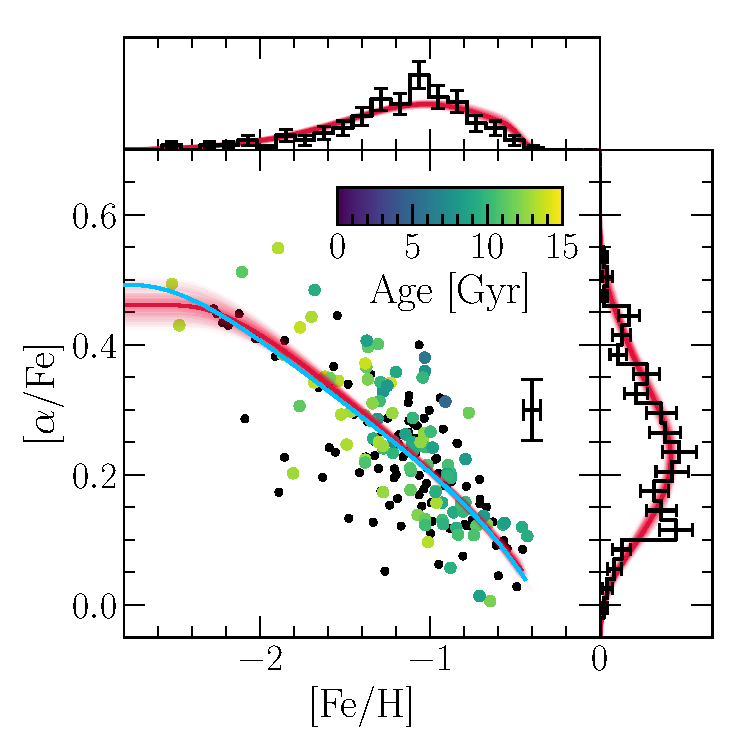
\includegraphics[scale = 0.5]{gsefit_afe_feh.pdf}
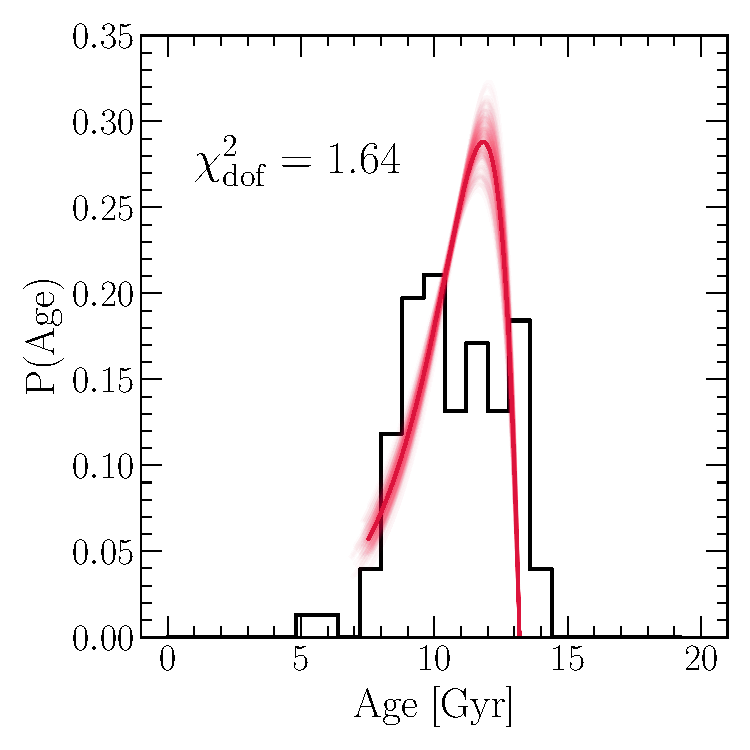
\includegraphics[scale = 0.42]{gsefit_agedist.pdf}
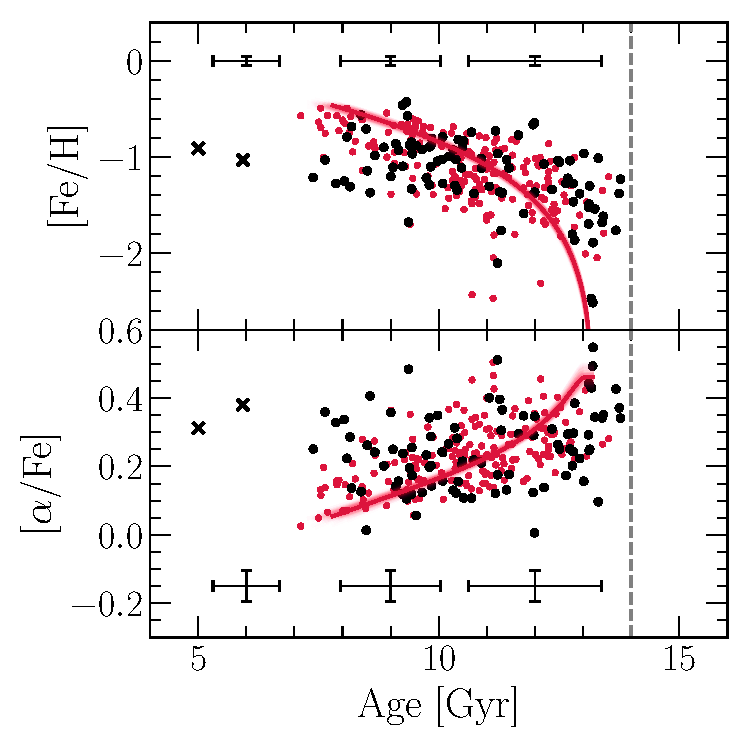
\includegraphics[scale = 0.42]{gsefit_amr.pdf}
\caption{
\textbf{Left}: The~\afe-\feh~plane and associated marginalized distributions.
Stars are colour-coded according to their age where available and are otherwise
plotted in black.
The best-fit chemical evolution track and distributions in~\afe~and~\feh~are
shown as solid red lines.
The median~\feh~and~\afe~errors of the sample are shown by the error bar to the
right of the data. 
\textbf{Middle}: The age distribution measured for our GSE sample (black) and
the best-fit age distribution based on the SFH of our model (red, solid).
We additionally plot the age distribution obtained when we convolve the best-fit
distribution with an uncertainty of~$\sigma(\log_{10}(\text{age}))$ including
the prior that age~$<$ 14 Gyr as in the H3 age measurements.
\textbf{Right}: The age-\feh~and age-\afe~relations of our GSE sample (black)
and our best-fit chemical evolution model (red).
The median~\feh,~\afe, and age uncertainties are shown by the error bars to the
left of the data in each panel.
We plot the two stars that we exclude from our fit as our black X's (see
discussion in~\S~\ref{sec:h3:gse}).
In all panels, we subsample 200 sets of parameter choices~$\{\theta\}$ from our
likelihood distribution (see Fig.~\ref{fig:gse_corner}) and plot their
predictions as high transparency lines to provide a sense of the fit precision
in the observed space.
}
\label{fig:gse_bestfit}
\end{figure*}

\begin{figure*}
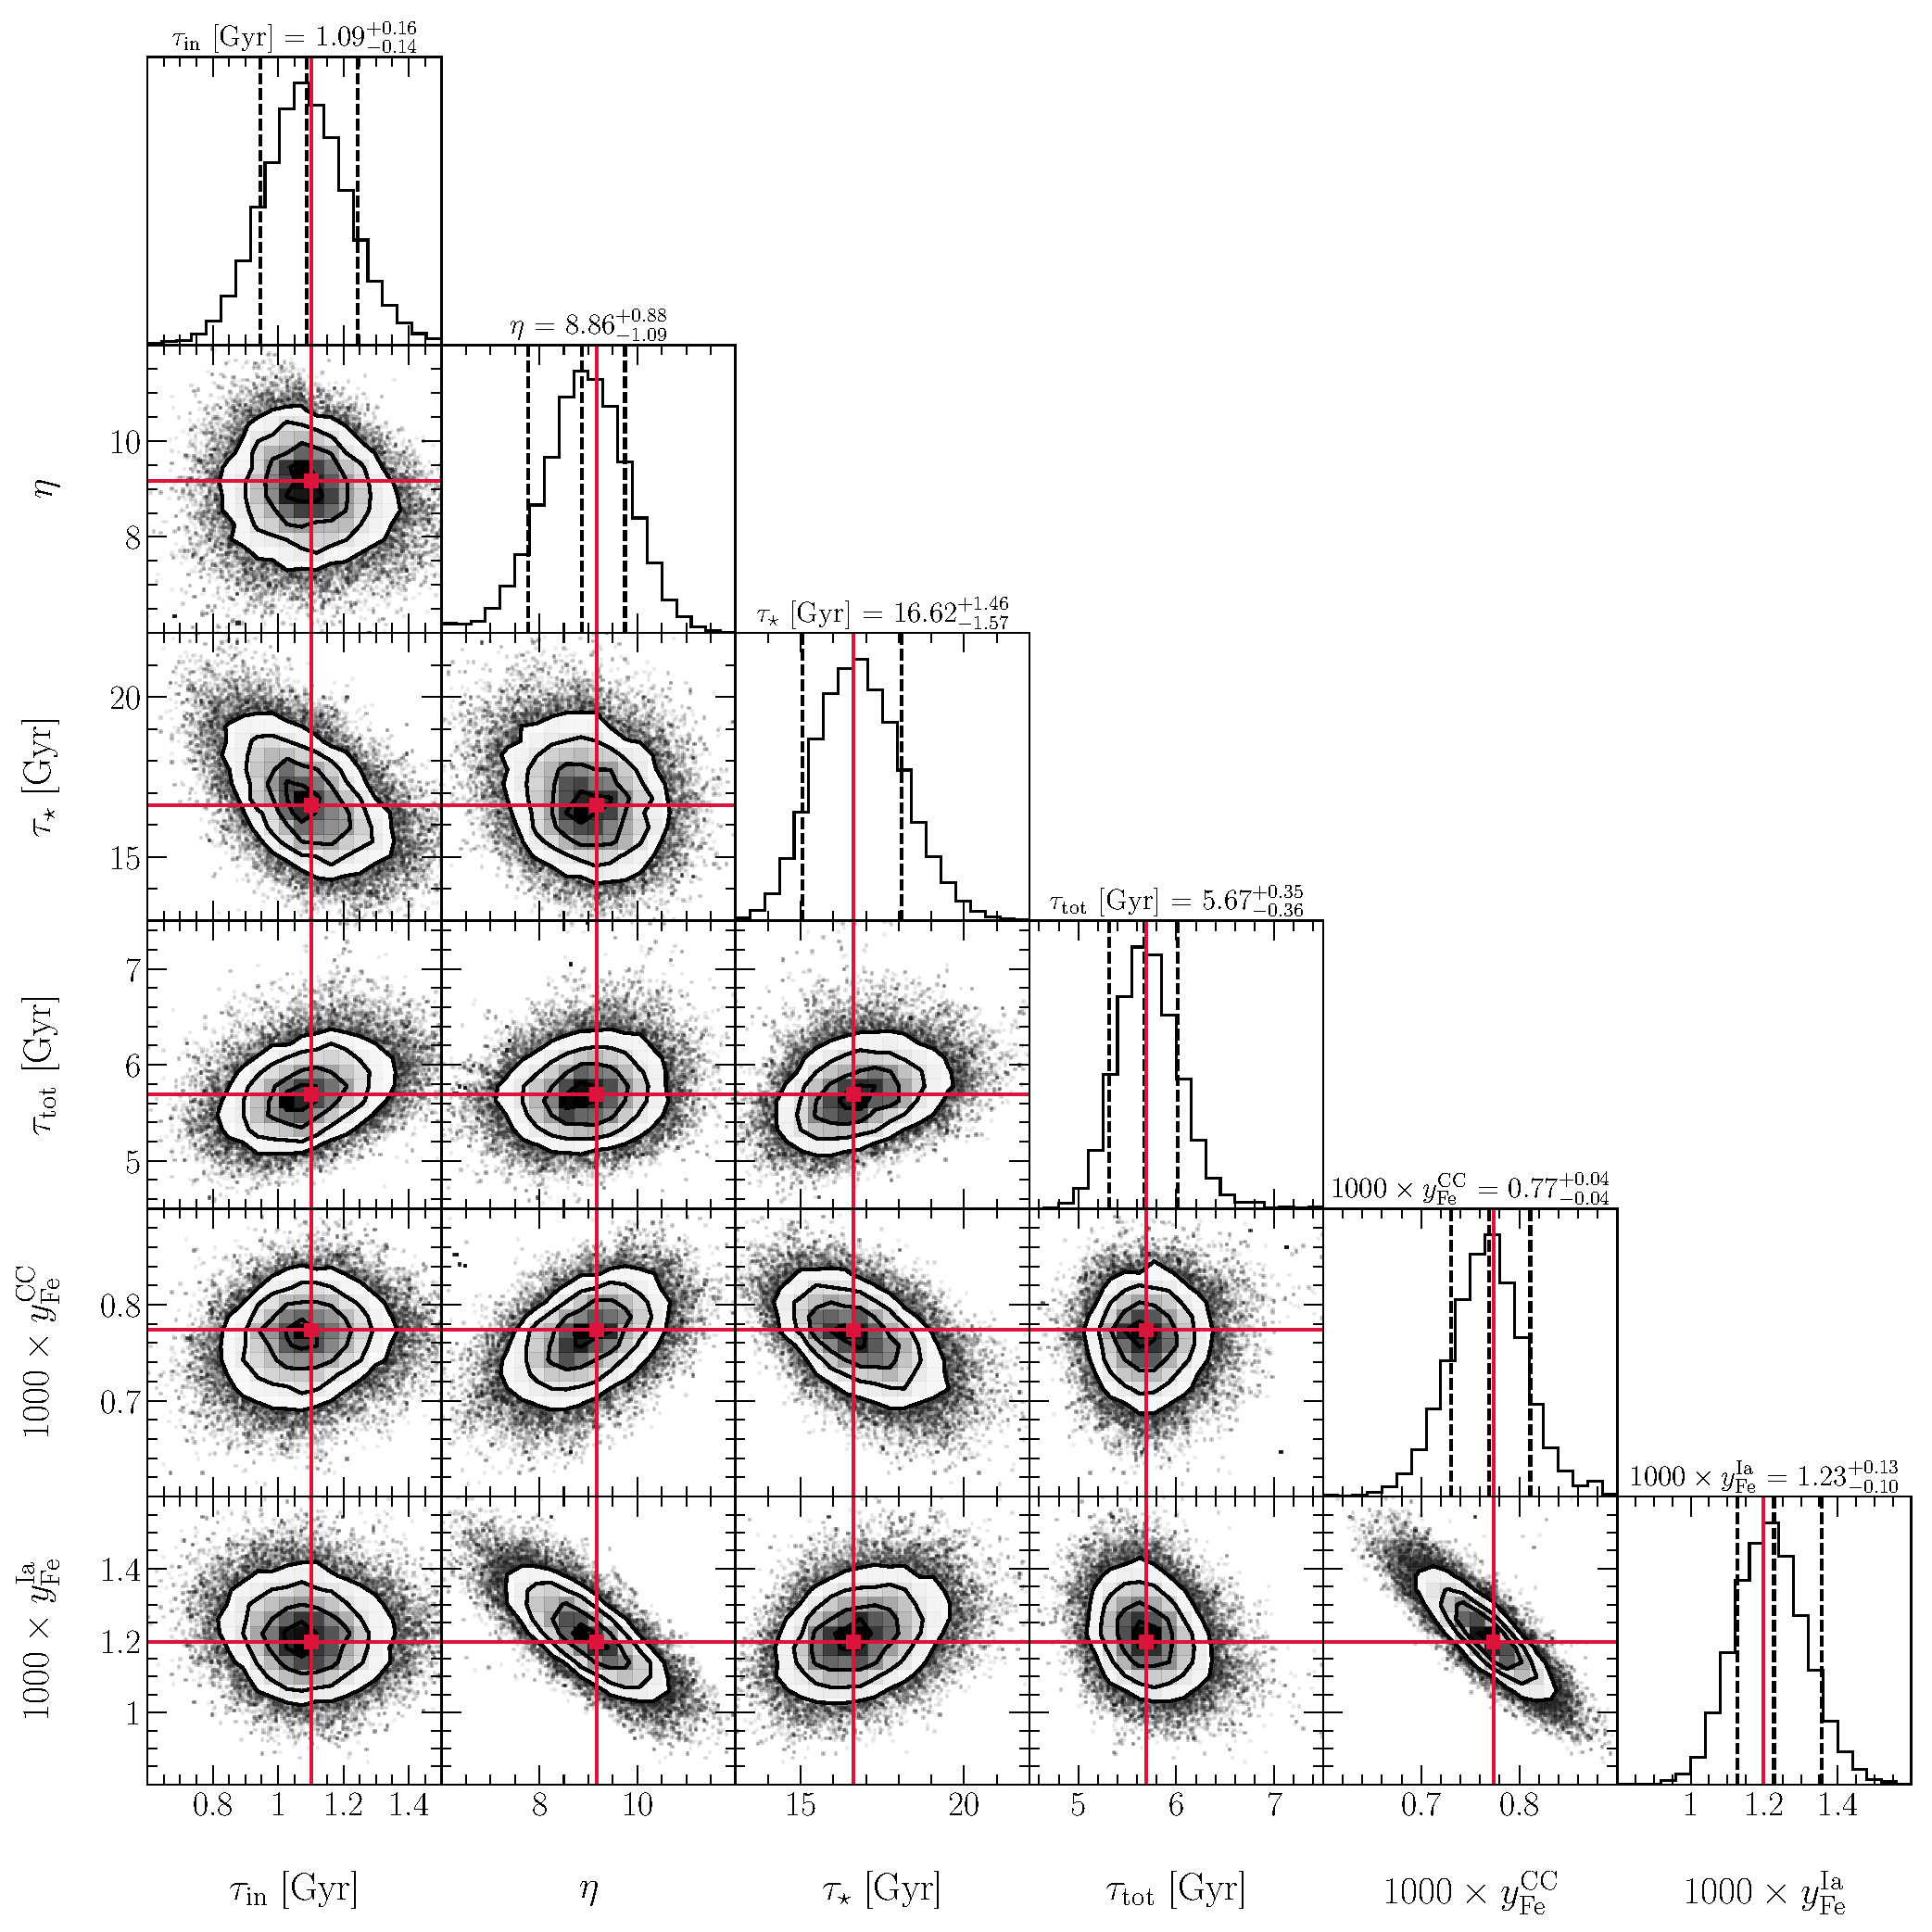
\includegraphics[scale = 0.45]{gsechem_102k4.pdf}
\caption{
The ``corner-plot'' showing the results of our fitting method applied to GSE
stars observed by the H3 survey.
We show the marginalized likelihood distributions in each parameter along with
their best-fit values and confidence intervals along the diagonal.
Below the diagonal, we show the 2-dimensional cross-sections of the
6-dimensional likelihood function.
Contrary to Fig.~\ref{fig:corner_fiducial}, red ``cross-hairs'' mark the
element of the Markov chain with the maximum statistical likelihood.
}
\label{fig:gse_corner}
\end{figure*}

\begin{itemize}

	\item Our sample from the GSE consists of 189 stars, 95 of which have
	age measurements.
	These stars span metallicities of~$\feh \approx -2.5$ to~$-0.4$ and
	$\afe \approx 0$ to $+0.55$.
	Abundance uncertainties range from~$\sim$0.02 to~$\sim$0.12 in
	both~\feh~and~\afe~with median values near~$\sim$0.05.
	Of the stars with age measurements, the youngest is~$\sim$5 Gyr old and the
	oldest is~$\sim$13.8 Gyr old.
	All inferred ages, however, incorporate a prior imposed by the H3 pipeline
	which requires all values to be below 14 Gyr, preventing the log-normal
	nature of age uncertainties from populating the~$\sim14 - 20$ Gyr range.
	Every age measurement has a statistical uncertainty below
	$\sigma(\log_{10}(\text{age})) = 0.05$, corresponding to a measurement
	precision of~$\lesssim$12\%.
	Due to the difficulty associated with measuring stellar ages both
	accurately and precisely (refs), we adopt this value of
	$\sigma(\log_{10}(\text{age})) = 0.05$ as the minimum uncertainty to
	account for any systematic errors that may be present.
	This consequently applies to the whole subset of our sample that has age
	measurements.

	\item The left panel of Fig.~\ref{fig:gse_bestfit} shows our sample in
	the~\afe-\feh~plane along with the associated marginalized distributions.
	The mode of the MDF is near~$\feh = -1$ and~$\afe = +0.25$, and the
	``knee'' associated with the onset of SNe ia enrichment is apparent
	near~$\feh \approx -2$, though there are only a few stars in our sample
	in this region of chemical space.
	Invoking the equilibrium arguments of~\citet{Weinberg2017}, the knee
	occurring at low metallicity and an MDF dominated by low metallicity stars
	is indicative, respectively, of slow star formation (i.e. high~$\tau_\star$)
	and a low equilibrium abundance due to strong outflows (i.e. high~$\eta$).
	This is expected for a dwarf galaxy progenitor where star formation is
	typically slow~\citep[e.g.][]{Hudson2015} and the gravitational potential
	well is shallow due to low stellar and halo masses.

	\item In the middle and right panels, we show the age distribution,
	age-\feh~relation, and age-\afe~relation.
	The age distribution is dominated by old stars ($\gtrsim$8 Gyr), consistent
	with previous studies of the GSE (refs).
	The truncation of the age distribution likely reflects the quenching of
	star formation in the GSE progenitor by ram pressure stripping at the time
	of its first infall into the Milky Way (refs).
	The age-metallicity relation (AMR), both age-\feh~and age-\afe, has a
	considerable amount of scatter, in large part because of the considerable
	age uncertainties compared to the abundance uncertainties.

	\item We note the presence of two outliers at ages of~$\sim$5 and 6 Gyr,
	marked by X's in the right panel.
	These stars have abundances typical of the rest of the GSE population but
	are anomalously young.
	It's likely that these are blue stragglers: stars which are thought to be
	made hotter and more luminous by accretion from a binary companion.
	As a result, they occupy a region of the CMD which is normally occupied by
	much younger, more massive stars, biasing their age measurements to low
	values~\citep[e.g.][]{Bond1971, Stryker1993}.
	We therefore omit these stars from our chemical evolution model fit to the
	GSE, including only those which are older than~$\sim$7 Gyr.

	\item The steadily sloped decline of~\afe~with increasing~\feh~and the
	approximately monotonic nature of the age-\feh~and age-\afe~relations
	incidicate a smooth SFH.
	If the GSE had experienced a burst in star formation at some point in its
	history, this would be accompanied by a sudden increase in~\afe~followed by
	a decline back toward the pre-burst value due to the temporarily perturbed
	ratio of CCSN and SN Ia rates~\citep{Johnson2020}.
	We therefore fit the GSE with a smooth evolutionary model, adopting the
	same exponential infall history as our mock samples explored
	in~\S~\ref{sec:mocks}.

\end{itemize}

\subsection{The Sagittarius Dwarf Spheroidal}
\label{sec:h3:sgr}

\end{document}

